\documentclass[12pt,letterpaper,fleqn]{article}

\usepackage[utf8]{inputenc}
\usepackage{tikz}
\usepackage[utf8]{inputenc}
\usepackage[T1]{fontenc}
\usepackage{amsmath}
\usepackage{amssymb}
\usepackage{multicol}
\usepackage{graphicx}
\usepackage{mdwlist}
\usepackage{ upgreek }
\usepackage{ stmaryrd }


\usepackage[dvipsnames]{xcolor}
\usepackage[most]{tcolorbox}

\usepackage{tabu}

\usepackage{mathtools}

\usepackage[top=1in, bottom=1in, left=1in, right=1in]{geometry}


\begin{document}

    \begin{titlepage}
        \centering
        {\scshape\LARGE Universidad Nacional Autónoma de México \par}
    
        \vspace{0.5cm}
        {\scshape\LARGE Facultad de Ciencias\par}
    
        \begin{center}
            \includegraphics[scale=.6]{assets/logo.png}
        \end{center}
    
        {\scshape\LARGE \textbf{Tarea 01}\par}
        
       \vspace{.5 cm}
    
        {\scshape Presentan\par}
        \begin{center}
            \begin{itemize}
                \centering
                \item Nelson Osmar Garcia Villa - 322190357
                \item Valeria Camacho Hernández - 322007273
                \item Mauricio Casillas Álvarez - 322196342
            \end{itemize}
        \end{center}
        
        \vspace{.5 cm}

        {\scshape Asignatura \par}
        \begin{center}
            Gráficas y Juegos 2025-2
        \end{center}

            
        \vspace{.5 cm}

        {\scshape Profesor \par}

        \begin{center}
            César Hernández Cruz
        \end{center}

        \vspace{.5 cm}
        
        {\scshape Ayudante \par}
        
        \begin{center}
        Iñaki Cornejo de la Mora
        \end{center}
        
        \vspace{.5 cm}

        {\scshape Fecha \par}
        \begin{center}
        Miércoles 12 de Febrero del 2025
        \end{center}
        
        \vfill
    \end{titlepage}
    
\begin{center}
    \LARGE{\textbf{Tarea 01}}
\end{center}
    \begin{enumerate}
  \item Dibuje todas las gráficas no isomorfas de cuatro vértices. Justifique
    brevemente por qué son todas, es decir, justifique por qu\'e la lista que
    exhibe es exhaustiva.
    
     \underline{Respuesta:}

        Son 11 gráficas no isomorfas con cuatro vértices. Para determinar todas las posibles gráficas, observamos que una gráfica de cuatro vértices se construye añadiendo o eliminando aristas entre los $\binom{4}{2} = 6$
        pares de vértices posibles.
 
\begin{figure}[h]
    \centering
\includegraphics[width=0.9\linewidth]{graficas_11.png} 
\end{figure}
Cada una de estas estructuras es no isomorfa a las demás, lo que garantiza que la lista es exhaustiva.



  \item Sean $G$ y $H$ gr\'aficas.
    \begin{enumerate}
        \item Demuestre que $G$ es isomorfa a $H$ si y s\'olo si $\overline{G}$
            es isomorfa a $\overline{H}$.
    \end{enumerate}
        \underline{Respuesta:} Sean \( G \) y \( H \) dos gráficas.
        \\
        
        \(\Rightarrow \text{Si } \overline{G} \cong \overline{H}, \text{ entonces } G \cong H.\)
            
        Por demostrar: \( G \cong H \).
        
        Supongamos que \( \overline{G} \cong \overline{H} \). Esto quiere decir que existe una función biyectiva \(\varphi: V(\overline{G}) \rightarrow V(\overline{H})\) que conserva la adyacencia y la no adyacencia.

        Si \( uv \in E(G) \), entonces \( uv \notin E(\overline{G})\). Como \( \varphi \) es un isomorfismo, sucede que \( \varphi(u)\varphi(v) \notin E(\overline{H}) \), lo que implica que \( \varphi(u)\varphi(v) \in E(H) \) (por definición de la operación complemento). Así, \( \varphi \) conserva la adyacencia entre \( G \) y \( H \). 
 
        Si \( uv \in E(\overline{G}) \), entonces \( uv \notin E(G) \). Como \( \varphi \) es un isomorfismo, sucede que \( \varphi(u)\varphi(v) \in E(\overline{H}) \), lo que implica que \( \varphi(u)\varphi(v) \notin E(H) \) (por definición de la operación complemento). Así, \( \varphi \) conserva la no adyacencia entre \( G \) y \( H \). 

        Por lo tanto,  \( \varphi \) preserva las adyacencias y las no adyacencias entre \( G \) y \( H \).
        \[\therefore G \cong H. \]
        
        \(\Leftarrow \text{Si } G \cong H, \text{ entonces } \overline{G} \cong \overline{H}.\)

        Por demostrar: \( \overline{G} \cong \overline{H} \).
            
        Supongamos que \( G \cong H \). Entonces existe una función biyectiva \(\varphi: V(G) \rightarrow V(H)\) que conserva la adyacencia y la no adyacencia.
            
        Si \( uv \notin E(G) \), entonces \( uv \in E(\overline{G}) \). Luego, como \( \varphi \) es un isomorfismo, sucede \( \varphi(u)\varphi(v) \notin E(H) \), lo que implica que \( \varphi(u)\varphi(v) \in E(\overline{H}) \) (por definición de de la operación complemento). Así, \( \varphi \) conserva la adyacencia entre \( \overline{G} \) y \( \overline{H} \). 
        
        Si \( uv \notin E(\overline{G}) \), entonces \( uv \in E(G) \). Luego, como \( \varphi \) es un isomorfismo, sucede \( \varphi(u)\varphi(v) \in E(H) \), lo que implica que \( \varphi(u)\varphi(v) \notin E(\overline{H}) \) (por definición de de la operación complemento). Así, \( \varphi \) conserva la no adyacencia entre \( \overline{G} \) y \( \overline{H} \). 

        Por lo tanto, \( \varphi \) conserva las adyacencias y las no adyacencias entre \( \overline{G} \) y \( \overline{H} \).  
        \[\therefore \overline{G} \cong \overline{H} \]
        
        Como \( G \cong H \) si y sólo si \( \overline{G} \cong \overline{H} \), queda demostrado.  \(\bigstar\)
        \\

    \begin{enumerate}
        \item Usando la definición de conexidad vista en clase, demuestre que
            si $G$ es inconexa, entonces $\overline{G}$ es conexa.   
        \end{enumerate}
        \underline{Respuesta:} Sea \( G \) una gráfica.
        
        Por demostrar: \( \text{Si } G \text{ es inconexa, entonces } \overline{G} \text{ es conexa} \).
        
        Supongamos que \( G \) es inconexa.  
        Entonces existe una partición de \( V \) en dos conjuntos disjuntos \( X \) y \( Y \), con \( X \cup Y = V \), tal que no hay aristas que conecten a \( X \) y \( Y \) en la gráfica \( G \).
        
        Ahora, el complemento de \( G \) es \( \overline{G} = (V, \overline{E}) \), donde  \(\overline{E} = \{ (u,v) \mid u, v \in V, u \neq v \text{ y } uv \notin E \}\). Es decir, \( \overline{G} \) tiene exactamente las aristas que en \( G \) no están  (por definición de la operación complemento).
        
        Entonces, como en \( G \) no hay aristas que conecten a \( X \) y \( Y \), en \( \overline{G} \) sí están (por definición de la operación complemento) todas las aristas entre  \( X \) y \( Y \). Así, cualquier vértice no conectado en \( G \), estará conectado en \( \overline{G} \), es decir, cualquier vértice de \( X \) está conectado con uno de \( Y \) en \( \overline{G} \). Es particular, si \( u \in X\) y \( v \in Y\), entonces estarán conectados en \(\overline{G}\), mientras que si \( uv \in X\) ó $Y$, entonces estarán conectados a través de un vértice que ya sea que este en $X$ ó $Y$, respectivamente. De esta manera, \(\overline{G}\) resulta en ser conexa. 
        
        Como $G$ es inconexa, entonces \( \overline{G}\) es  conexa y queda demostrado. \(\bigstar\)

  \item Sea $D$ una digráfica.   Utilizando un análogo para digráficas de
    las matrices de incidencia, demuestre que
    \[
      \sum_{v \in V_D} d^+(v) = \sum_{v \in V_D} d^-(v) = |A_D|.
    \]
    \underline{Respuesta:} 
    Por demostrar: La suma del número de aristas que salen de un vértice $v$ (exgrados) es igual a la suma del número de aristas que entran a un vértice $v$ (ingrados), y ambas por separado son igual al número total de aristas en la gráfica D.
    
    1) Definimos la matriz de incidencia para exgrados como $M^+$, donde cada fila representa un vértice y cada columna representa una arista. Sus valores son:

    \[M^+_{ij} =
    \begin{cases}
    1, & \text{si la arista } j \text{ sale del vértice } i, \\
    0, & \text{en otro caso}.
    \end{cases}\]

    El exgrado $d^+(v)$, de un vértice $i$ es el número de aristas que salen de $v$ y para obtenerlo, se suman los valores de su fila, como:
    \[ d^+(i) = \sum_{j=1}^{|A_D|} M^+_{ij}\]

    Luego, para saber el exgrado de todos los vértices, es decir, si sumamos todos los vértices de la gráfica, tenemos:
    \[ \sum_{i=1}^{|V_D|} d^+(i) = \sum_{i=1}^{|V_D|} \sum_{j=1}^{|A_D|} M^+_{ij} \]

    Cada arista tiene exactamente un vértice de origen, lo que significa que cada columna de la matriz $M^+$ tiene exactamente un $1$. Esto implica que la suma sobre todas las filas cuenta cada arista exactamente una vez, por lo que:
    \[ \sum_{i=1}^{|V_D|} d^+(i) = |A_D|0 \]

    2) Ahora definimos la matriz de incidencia para ingrados, $M^{-}$, con valores:
    \[ M^{-}_{kj} = \begin{cases}
    1, & \text{si la arista } j \text{ entra al vértice } k, \\
    0, & \text{en otro caso}.
    \end{cases} \]
    
    El ingrado de un vértice $k$ se obtiene sumando los valores de su fila: \[ d^{-}(k) = \sum_{j=1}^{|A_D|} M^{-}_{kj} \]

    Si sumamos sobre todos los vértices $k$, obtenemos: \[
    \sum_{k=1}^{|V_D|} d^{-}(k) = \sum_{k=1}^{|V_D|} \sum_{j=1}^{|A_D|} M^{-}_{kj} \]

    Cada arista tiene exactamente un vértice de destino, lo que significa que cada columna de $M^{-}$ tiene exactamente un $1$, por lo que: \[ \sum_{k=1}^{|V_D|} d^{-}(k) = |A_D| \]
    
    De esta manera, las sumas coinciden con el número de aristas porque se está contando cada una de las contribuciones de cada arista a los exgrados y a los ingrados, al recorrer toda la matriz con las sumas.

    Por lo tanto, \( \sum_{v \in V_D} d^+(v) = \sum_{v \in V_D} d^-(v) = |A_D|.
    \) \(\bigstar\)

  \item  Sea $n$ un entero positivo. Definimos a la {\em Retícula Booleana},
    $BL_n$, como la gráfica cuyo conjunto de vértices es el conjunto de todos
    los posibles subconjuntos de $\set{1, \cdots, n}$, donde dos subconjuntos
    $X$ y $Y$ son adyacentes si y sólo si su diferencia simétrica tiene
    exactamente un elemento.
    \begin{enumerate}
      \item Dibuje $BL_1, BL_2, BL_3$ y $BL_4$.
        \begin{center}
            BL1 \end{center}
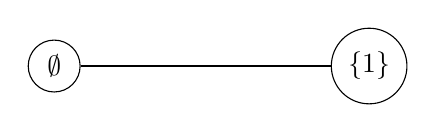
\begin{tikzpicture}

  \node[draw, circle] (0) at (0,0) {$\emptyset$};
  \node[draw, circle] (1) at (4,0) {$\{1\}$};
  \draw[thick] (0) -- (1);
\end{tikzpicture}

\begin{center}
            BL2 \end{center}
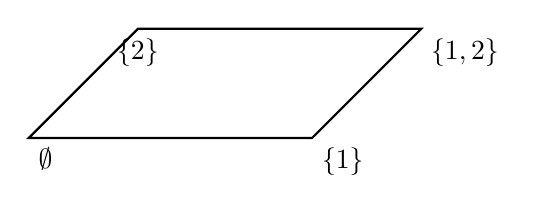
\begin{tikzpicture}[scale=6] 

\coordinate (2) at (0.2,0.2,0.2);
\coordinate (12) at (0.8,0.2,0.2);
\coordinate (0) at (0.2,0.2,0.8);
\coordinate (1) at (0.8,0.2,0.8);

\draw[thick] (0) -- (1) -- (12) -- (2) -- cycle;

\node at (2) [below] {$\{2\}$};
\node at (12) [below right] {$\{1,2\}$};
\node at (0) [below right] {$\emptyset$};
\node at (1) [below right] {$\{1\}$};

\end{tikzpicture}

\begin{center}
            BL3 \end{center}
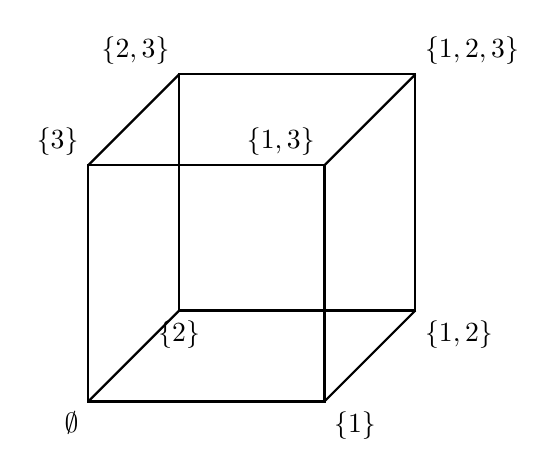
\begin{tikzpicture}[scale=5]

\coordinate (2) at (0.2,0.2,0.2);
\coordinate (12) at (0.8,0.2,0.2);
\coordinate (123) at (0.8,0.8,0.2);
\coordinate (23) at (0.2,0.8,0.2);
\coordinate (0) at (0.2,0.2,0.8);
\coordinate (1) at (0.8,0.2,0.8);
\coordinate (13) at (0.8,0.8,0.8);
\coordinate (3) at (0.2,0.8,0.8);

\draw[thick] (2) -- (12) -- (123) -- (23) -- cycle;
\draw[thick] (0) -- (1) -- (13) -- (3) -- cycle;
\draw[thick] (2) -- (0);
\draw[thick] (12) -- (1);
\draw[thick] (123) -- (13);
\draw[thick] (23) -- (3);

\node at (2) [below] {$\{2\}$};
\node at (12) [below right] {$\{1,2\}$};
\node at (123) [above right] {$\{1,2,3\}$};
\node at (23) [above left] {$\{2,3\}$};
\node at (0) [below left] {$\emptyset$};
\node at (1) [below right] {$\{1\}$};
\node at (13) [above left] {$\{1,3\}$};
\node at (3) [above left] {$\{3\}$};
\end{tikzpicture}

\begin{center}
            BL4 \end{center}


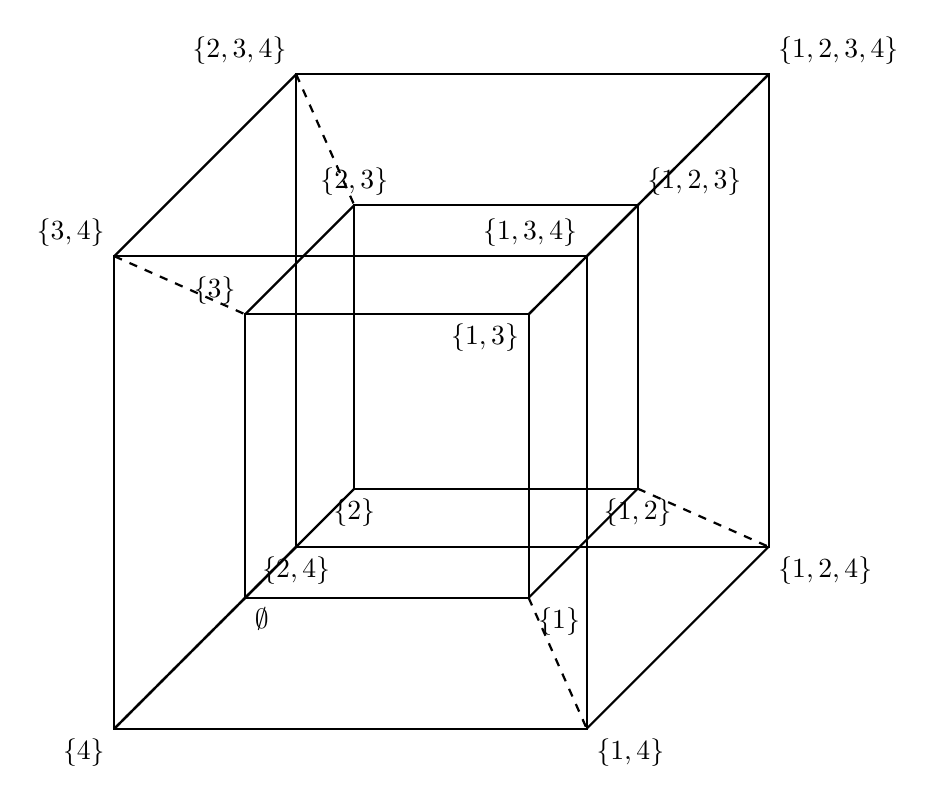
\begin{tikzpicture}[scale=6]

\coordinate (24) at (0,0,0);
\coordinate (124) at (1,0,0);
\coordinate (1234) at (1,1,0);
\coordinate (234) at (0,1,0);
\coordinate (4) at (0,0,1);
\coordinate (14) at (1,0,1);
\coordinate (134) at (1,1,1);
\coordinate (34) at (0,1,1);


\coordinate (2) at (0.2,0.2,0.2);
\coordinate (12) at (0.8,0.2,0.2);
\coordinate (123) at (0.8,0.8,0.2);
\coordinate (23) at (0.2,0.8,0.2);
\coordinate (0) at (0.2,0.2,0.8);
\coordinate (1) at (0.8,0.2,0.8);
\coordinate (13) at (0.8,0.8,0.8);
\coordinate (3) at (0.2,0.8,0.8);

% A del cubo exterior
\draw[thick] (24) -- (124) -- (1234) -- (234) -- cycle;
\draw[thick] (4) -- (14) -- (134) -- (34) -- cycle;
\draw[thick] (24) -- (4);
\draw[thick] (124) -- (14);
\draw[thick] (1234) -- (134);
\draw[thick] (234) -- (34);

% A del cubointerior
\draw[thick] (2) -- (12) -- (123) -- (23) -- cycle;
\draw[thick] (0) -- (1) -- (13) -- (3) -- cycle;
\draw[thick] (2) -- (0);
\draw[thick] (12) -- (1);
\draw[thick] (123) -- (13);
\draw[thick] (23) -- (3);

\draw[thick, dashed] (1) -- (14);
\draw[thick, dashed] (0) -- (4);
\draw[thick, dashed] (24) -- (4);
\draw[thick, dashed] (34) -- (3);
\draw[thick, dashed] (12) -- (124);
\draw[thick, dashed] (234) -- (23);
\draw[thick, dashed] (13) -- (134);
\draw[thick, dashed] (1234) -- (123);

% V cubo exterior
\node at (24) [below ] {$\{2,4\}$};
\node at (124) [below right] {$\{1,2,4\}$};
\node at (1234) [above right] {$\{1,2,3,4\}$};
\node at (234) [above left] {$\{2,3,4\}$};
\node at (4) [below left] {$\{4\}$};
\node at (14) [below right] {$\{1,4\}$};
\node at (134) [above left] {$\{1,3,4\}$};
\node at (34) [above left] {$\{3,4\}$};

% V cubo interior
\node at (2) [below] {$\{2\}$};
\node at (12) [below] {$\{1,2\}$};
\node at (123) [above right] {$\{1,2,3\}$};
\node at (23) [above] {$\{2,3\}$};
\node at (0) [below right] {$\emptyset$};
\node at (1) [below right] {$\{1\}$};
\node at (13) [below left] {$\{1,3\}$};
\node at (3) [above left] {$\{3\}$};
\end{tikzpicture}
      \item Determine $|V_{BL_n}|$ y $|E_{BL_n}|$. (Demuestre su respuesta.)\\
      \\
      \underline{Respuesta:}
       \begin{enumerate}
           \item $|V_{BL_n}|$, la característica de los vértices en la gráfica, es que el conjunto de los vértices es el conjunto de todos los posibles subconjuntos.Esto es básicamente la definición del conjunto Potencia $($recordando que este agrega el $\emptyset$$)$.\\
            Dicho conjunto potencia tiene una formula la cual se estable como $2^n$, n representa en este caso los números enteros positivos .\\
            Por lo tanto $|V_{BL_n}|$ = $2^n$ \\
            \item $|E_{BL_n}|$, Recordando la formula para sacar el máximo número de aristas en una gráfica es: 
            \begin{equation}
         \hspace{4.5cm} \frac{n*(n-1)}{2}
        \end{equation}
            este caso solo se cumple si y solo si la gráfica es completa, ya que se relaciona con todos los vértices n excepto consigo de ahí viene $(n-1)$, pero eso es una condición de dicha fórmula, sabiendo que los vértices $|$VBLn$|$ se obtiene por $2^n$, respetando la condición que es su diferencia simétrica forzosamente de un solo elemento, viendo que tanto $(n-1)$ y $2^n$ son condiciones podemos sustituirlas en la formula principal quedando:
            \begin{equation}
            \hspace{5cm} \frac{n*(2^n)}{2}
        \end{equation}
            de esta forma podemos conocer el número de aristas en ${BL_n}$.
       \end{enumerate}    
      \item Demuestre que $|E_{BL_n}|$ es bipartita para cualquier $n \in \mathbb{Z}^+$.
        \end{enumerate}
        \raggedright
        \underline{Respuesta:}
    \\
        $Bl_n$ es el conjunto de vértices de todos los subconjuntos, dos vertices X y Y son adyacentes si su diferencia simetrica tiene un elemento. \\
        $\rightarrow$ Sea $n \in \mathbb Z^+$\\
        \underline{Dem.} Que $Bl_n$ es bipartita \\
        $\rightarrow$Sea $Bl_n$ una grafica bipartita si podemos dar una partición en dos conjuntos, donde no haya aristas dentro del mismo conjunto de vertices. \\Siguiendo la definición podemos separar los subconjuntos en conjuntos par e impar: \medskip  \\
        $X = \{ x \in V \mid |x| \text{ es par}\} $ \hspace{1.5111 cm}(suconjuntos de tamaño par)\\
        $Y = \{ y \in V \mid |y| \text {es impar}\}$ \hspace{1.3 cm}(subconjuntos de tamaño impar)\medskip \\
        Esto implica que X y Y sean adyacentes por la diferencia simétrica en la que siempre habrá un solo elemento, conecta un vértice de tamaño par con uno de tamaño impar\\
        Como los vértices admiten una partición en la que dentro de los conjuntos X y Y no haya aristas y solo exista aristas para unir un conjunto con otro cuando haya un solo elemento en la diferencia simétrica dada la definición de adyacencia en $Bl_n$ \\
        \underline{Por lo tanto $BL_n$ es bipartita}
        
  \item El algoritmo de Euclides es uno de los  algoritmos más antiguos que sigue
    siendo usado hoy en día. Este se basa en el hecho que el máximo común divisor
    de dos números $a$ y $b$ con $a > b$, es igual al máximo común divisor de
    $a \% b$ (el residuo de $a$ entre $b$) y $b$.

    Escribe el pseudocódigo del algoritmo de Euclides en su versión iterativa y
    su versión recursiva.
\newpage    
\end{enumerate}
    \underline{Respuesta:}
\\
    - Iterativo:
    \\
    Input: Dos números a y b, donde a tiene que ser mayor que b .
    \\
    Output: Máximo Común Divisor (MCD)
    \\
    
    \begin{enumerate}
        \item a $\leftarrow$ número
        \item b $\leftarrow$ número
        \item prov $\leftarrow$ b
        \item If $a$ mayor que $b$ then
        \item  \hspace{0.5cm} while b diferente de 0 do
        \item \hspace{1cm} prov $\leftarrow$ b
        \item \hspace{1cm} b $\leftarrow$ a modulo b
        \item \hspace{1cm} a $\leftarrow$ prov
        \item Return a
    \end{enumerate} 
    \\ 
    - Recursivo
    \\
    Input: Dos números a y b, donde a tiene que ser mayor que b .
    \\
    Output: Máximo Común Divisor (MCD)
    \\ 
    \hspace{0.3cm} Euclides (a,b)
    \begin{enumerate}
        \item If b es igual de 0 then
        \item \hspace{0.5cm} Return a
        \item Return a $\leftarrow$ b, Euclides (a modulo b)
    \end{enumerate}
\bigskip
\subsection*{Punto Extra}

\begin{enumerate}
  \item Sea $G = [X, Y]$ una gráfica bipartita con $|X| = r$ y $|Y| = s$.
    \begin{enumerate}
      \item Demuestre que $|E| \le rs$.
      \\
      \underline{Respuesta:} Por definición, sabemos que $E$ está conectado a un vértice de $X$ con un vértice de $Y$.
      \\
      El número máximo de aristas ocurre cuando cada vértice de $X$ está conectado con cada vértice de $Y$. Esto también forma una gráfica bipartita completa, donde el número de aristas es $rs$.
      \\
      Entonces, esto significa que, para cualquier gráfica bipartita, el número de aristas $\lvert E \rvert$ no excede $rs$.
      \\
      Por lo tanto, se demostró que $\lvert E \rvert \leq rs$.
      \item Deduzca que $|E| \le \frac{|V|^2}{4}$.
      \\
      \underline{Respuesta:} Sabemos que a) es verdadero, es decir, que $\lvert E \rvert \leq rs$. Además, sabemos que $\lvert V \rvert = r + s$. Se busca demostrar que $rs \leq \frac{(r+s)^2}{4}$. 
      \\
      Se puede usar la desigualdad media aritmética-media geométrica (MA-GM), que nos dice que $\frac{a+b}{2} \geq \sqrt{ab}$. Aplicando esto a $r$ y $s$, tenemos:
        \[
        \frac{r+s}{2} \geq \sqrt{rs}.
        \] 
    Elevando ambos lados al cuadrado, obtenemos:
        \[
        \left(\frac{r+s}{2}\right)^2 \geq rs.
        \]
    Reorganizando, esto implica que:
        \[
        \frac{(r+s)^2}{4} \geq rs.
        \]
    Como ya sabemos que $\lvert E \rvert = rs$, esto implica que:
        \[
        \lvert E \rvert \leq \frac{\lvert V \rvert^2}{4}.
        \]
      \item Describa a las gráficas bipartitas que cumplen la igualdad en el inciso anterior. Justifique su respuesta.
      \\
        \underline{Respuesta:} Las gráficas bipartitas completas son aquellas que cumplen la igualdad, donde los dos conjuntos de vértices $X$ y $Y$ tienen el mismo tamaño, esto se debe a que deben cumplir la igualdad en la desigualdad MA-GM. Esta igualdad sólo se cumple si $r = s$, es decir, que los dos conjuntos de vértices deben tener el mismo número de elemento y que sea una gráfica completa, cuando $r = s$ esto hace que la gráfica bipartita sea completa. 
    \end{enumerate}
\end{enumerate}
\end{document}

